\section{GRAIL Translation Pipeline}
\label{sec:system}

\begin{figure}[t]
    \centering
    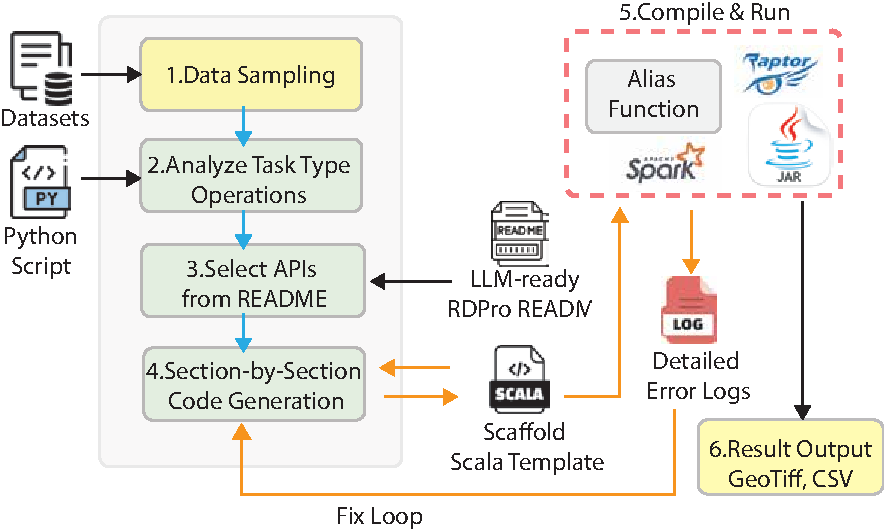
\includegraphics[width=\columnwidth]{figures/GRAIL.pdf}
    \caption{GRAIL translation system overview.}
    \Description{
    % AI-generated
    Flowchart titled ``GRAIL translation system overview.'' Inputs on the left are datasets and a Python script. The main pipeline has four steps: (1) data sampling, (2) analyze task type and operations, (3) select APIs from README, and (4) section-by-section code generation. An ``LLM-ready RDPro README'' feeds into API selection, and a ``scaffold Scala template'' supports code generation. The generated Scala code is then sent to step (5) compile and run, which includes alias functions and the Raptor, Spark, and Java/JAR environments. Compilation produces detailed error logs, which feed back into code generation through a fix loop. Successful execution produces step (6) result output, shown as GeoTIFF and CSV. Arrows indicate the end-to-end workflow and iterative debugging loop.
    }
    \label{fig:grail}
\end{figure}
Figure~\ref{fig:grail} illustrates the GRAIL pipeline. The system accepts either a Python script or a plain-text task description and produces an executable RDPro Scala program. GRAIL decomposes translation into four stages: task analysis, section planning, section-by-section generation, and iterative repair.

\textbf{Task Analysis.}
GRAIL converts the input, either Python script or plain-text, into a structured intermediate representation that captures the task type and required geospatial operations. Translating the code into this representation reduces the risk of mis-translating source-language function calls directly into the target library.

\textbf{Section Planning.}
A planner analyzes the task and selects relevant sections from the LLM-ready documentation, then instantiates them using a \emph{scaffold file} that defines the general structure of a geospatial job. The scaffold covers six logical stages: \textsc{LoadData} specifies raster and vector inputs; \textsc{TypeCheck} validates pixel types to prevent casting errors; \textsc{SpatialCheck} ensures all datasets share a consistent geospatial extent; \textsc{Transform} handles raster-only preparation; \textsc{RasterVectorJoin} materializes the join between raster and vector data; and \textsc{Analytics} computes the final result, whether a histogram over raster data or an aggregated statistic from the join. Sections irrelevant to the inferred workflow are pruned before generation begins.

\textbf{Section-by-Section Generation.}
Each section is generated sequentially within a LangGraph loop. The prompt for each section incorporates the relevant API documentation fragments retrieved for that section, along with a section contract that specifies required API calls, input variables, expected output formats, and forbidden patterns. It also includes the current scaffold state, including variable summaries from preceding sections. This shared context allows later sections to build upon results generated in earlier sections.

\textbf{Validation and Repair.}
After each candidate section is generated, the pipeline applies four validation layers covering a scope check, a deterministic contract check, an LLM semantic review, and full Spark compilation and submission. If any layer fails, targeted repair feedback is assembled from the detected issues and injected into the next prompt, retrying only the failing section up to five rounds. Once all sections pass, a final whole-program review checks cross section invariants before writing the completed Scala program to disk.